\documentclass[oneside,senior,etd]{BYUPhysForDegree}

\usepackage[utf8]{inputenc}
\usepackage{rotating} 

% MY PACKAGES
\usepackage{indentfirst}

\usepackage[russian]{babel}
\usepackage{amsfonts} % Пакеты для математических символов и теорем
\usepackage{amstext}
\usepackage{amssymb}
\usepackage{amsthm}
\usepackage{graphicx} % Пакеты для вставки графики
\usepackage{subfig}
\usepackage{color}
\usepackage[unicode]{hyperref}
\usepackage[nottoc]{tocbibind} % Для того, чтобы список литературы отображался в оглавлении
\usepackage{algorithmic} % Для записи алгоритмов в псевдокоде
\usepackage{algorithm}
\usepackage{verbatim} % Для вставок заранее подготовленного текста в режиме as-is
\usepackage{listings}

\usepackage{commath}
\newcommand\Tau{\mathcal{T}}
\newcommand{\R}{\mathbb{R}}
\usepackage{color}
\usepackage[colorinlistoftodos, prependcaption]{todonotes}
\usepackage{multirow}
\newcommand*{\MyIndent}{\hspace*{0.2cm}}%

\Chair{Кафедра суперкомпьютеров и квантовой информатики}
\Lab{~}
\Year{2023}
  \Month{}
  \City{Москва}
  \AuthorText{Автор}
  \Author{Кучеров Василий Дмитриевич}
  \AuthorEng{}
  \AcadGroup{323}
  % Если вы не Пупкин Василий Иванович, то скопируйте себе этот проект через меню и уже потом правьте
  \TitleTop{Анализ влияния выбора функции потерь на}
  %\TitleMiddle{}
  \TitleBottom{эффективность обучения по нескольким примерам} % leave empty if you don't need it
  \TitleTopEng{}
  \TitleBottomEng{} % leave empty if you don't need it  
  \docname{Курсовая работа}
  %\docname{Выпускная квалификационная работа}
  %\docname{Магистерская диссертация}
  \Advisor{Буряк Дмитрий Юрьевич}  
  \AdvisorDegree{к.ф.-м.н.}
  % \Consultant{}
  % \ConsultantDegree{}
  
% \Abstract{Краткое описание задачи и основных результатов, мотивирующее прочитать весь текст}
% \AbstractEng{Abstract}


%%%% DON'T change this. It is here because .sty does not support cyrillic cp properly %%%%
\University{Московский государственный университет имени М.В.Ломоносова}
\Faculty{Факультет вычислительной математики и кибернетики}
\GrText{гр.}
\AdvisorText{Научный руководитель}
% \ConsultantText{}
% \AbstractText{}

\begin{document}
\fixmargins
\makepreliminarypages

\oneandhalfspace

\tableofcontents

\section{Введение}
\label{sec:Chapter0} \index{Chapter0}

\par
За последнее время с помощью машинного обучения были достигнуты значительные успехи во многих областях, начиная от распознавания изображений и заканчивая автопилотами.  Обучаясь на больших наборах данных, модель способна качественно обобщать их на новые примеры. Однако сбор и маркировка таких больших датасетов может оказаться времязатратной и дорогостоящей задачей, особенно для приложений, требующих уникальных данных или связанных с конфиденциальной информацией.

Среди таких приложений можно выделить следующие:
\begin{itemize}
    \item Распознавание ключевых слов (Keyword spotting) \cite{FSLKeywordSpotting}. При использовании в системах умного дома или голосовых ассистентах для добавления новых комманд нельзя заставить пользователя наговаривать сотни раз одни те же реплики..
    % https://arxiv.org/pdf/2210.02732.pdf
    \item Верификация по биометрии \cite{FSLBiometricVerification}: распознавание отпечатков пальцев, лица или голоса владельца. Возникает аналогичная проблема малого количества экземпляров, предоставляемых пользователем.
    % https://arxiv.org/pdf/2211.06761.pdf
    \item Поиск лекарств, основанный на подборе молекул \cite{FSLDrugDiscovery}: из за сложности синтеза или возможной токсичности обычно собирается только небольшое количество реально созданных и изученных молекул - кандидатов. На основе таких кандидатов требуется подобрать безопасный и более активный аналог.
\end{itemize}

\par
С целью решения данной проблемы появился подраздел машинного обучения - обучение по нескольким примерам (Few Shot Learning или FSL \cite{FSLsurvey}). В отличие от традиционного машинного обучения, в задачах FSL обучение производится всего по нескольким примерам, что дает возможность применять нейронные сети там, где раньше это было невозможно. Поскольку стандартные алгоритмы обучения нейронных сетей в условиях недостатка примеров будут приводить к переобучению, актуальной проблемой является разработка эффективных алгоритмов для FSL.

\par
Данная работа посвящена исследованию подходов к повышению эффективности обучения нейронных сетей при решении задачи FSL. 
 % Введение
\section{Обзор современных подходов}
\label{sec:Chapter1} \index{Chapter1}
\subsection{Обучение по нескольким примерам}

Поставим задачу FSL формально:  Пусть $R$ - ожидаемый риск; $\mathcal{H}$ - пространство гипотез; $\hat{h}$ - функция, минимизирующая ожидаемый риск; $h^*$ - функция в $\mathcal{H}$, минимизируящая ожидаемый риск; $h_I$ - функция в $\mathcal{H}$, минимизирующая эмпирический риск. Тогда общую ошибку можно представить в виде \cite{FSLsurvey}:

\large
$$
\mathbb{E}\left[R\left(h_I\right)-R(\hat{h})\right]=\underbrace{\mathbb{E}\left[R\left(h^*\right)-R(\hat{h})\right]}_{\mathcal{E}_{\text {app }}(\mathcal{H})}+\underbrace{\mathbb{E}\left[R\left(h_I\right)-R\left(h^*\right)\right]}_{\mathcal{E}_{\text {est }}(\mathcal{H}, I)}
$$

\normalsize
$\mathcal{E}_{\text {app }}$ - ошибка приближения (approximation), показывающая насколько хорошо могут функции в $\mathcal{H}$ аппроксимировать $\hat{h}$; $\mathcal{E}_{\text {est }}$ - ошибка расчета (estimation) показывает насколько хорошо мы можем приблизиться к $h^*$ в $\mathcal{H}$, минимизируя эмпирический риск.

\begin{figure}[h!]
\caption{Влияние размера обучающей выборки $I$ на $h_I$}
\centering
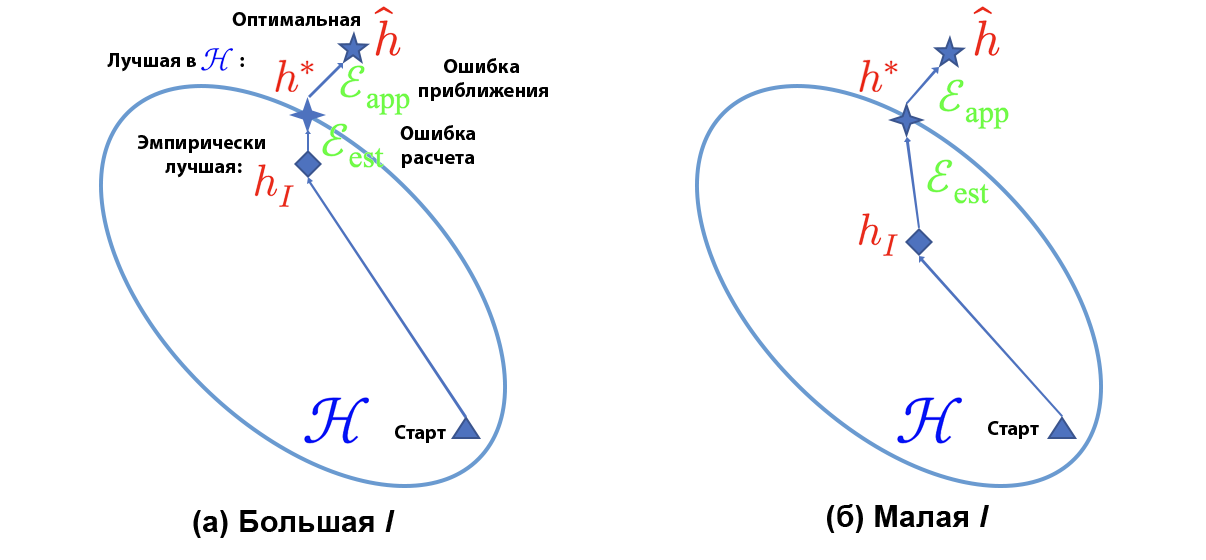
\includegraphics[width=16cm]{Images/H_largesmall_I_rus_noback.png}
\label{fig:H_largesmall_I_rus_noback}
\end{figure}

\begin{figure}[h!]

\centering
\end{figure}

\newpage

Используя некоторые предварительные знания о задаче можно выделить три подхода (Рис. \ref{fig:FSL_taxomony_rus_noback}) к уменьшению $\mathcal{E}_{\text {est }}$ \cite{FSLsurvey}: 
\begin{itemize}
    \item \textbf{Данные}. Увеличение обучающей выборки за счет преобразования объектов заданного датасета \cite{ReviewShareddensities, ReviewDeltaEncoder, ReviewLowShotVisual, ReviewOneShotSceneLocations, ReviewFeatureSpaceTransfer}, использования объектов из неразмеченных \cite{Review, ReviewLowShotDiffusion, ReviewStepwiseLearning}, слаборазмеченных датасетов или похожих датасетов \cite{ReviewStepwiseLearning, ReviewGenerativeAdversalNets, ReviewLowShotAugmentationNets}.
    \item \textbf{Модель}. Упрощение пространства гипотез $\mathcal{H}$. Тогда в новом пространстве $\Tilde{\mathcal{H}}$ имеющейся обучающей выборки будет достаточно для обучения. Различают многозадачное обучение \cite{ReviewMultitaskLearning, ReviewSurveyMultiTask, ReviewDeepLearning}, обучение эмбеддингов \cite{ReviewConvolutionArchitectureEmbedding, ReviewDifferentialGeometry}, обучение с внешней памятью \cite{ReviewNeuralTuringMachines, ReviewKeyValueMemory, ReviewEndToEndMemory,  ReviewMemoryNetworks}  и генеративное моделлирование \cite{ReviewNeuralStatistician, ReviewConceptLearning, ReviewFewShotAutoregressive, ReviewOneShotGeneralization}.
    \item \textbf{Алгоритм}. Выбор хорошей стартовой точки для обучения или добавление дополнительного шага в процессе обучения помимо шага минимизатора эмпирического риска. Выделяют такие методы, как уточнение существующих параметров \cite{ReviewOneShotVideoSegmentation}, уточнение мета-обученных параметров \cite{ReviewMetaLearningFastAdaptation} и обучение оптимизатора \cite{ReviewGradientDescendDouble, ReviewOptimizationModelFewShot}.
\end{itemize}

\begin{figure}[!h]
\caption{Схема подходов в FSL}
\centering
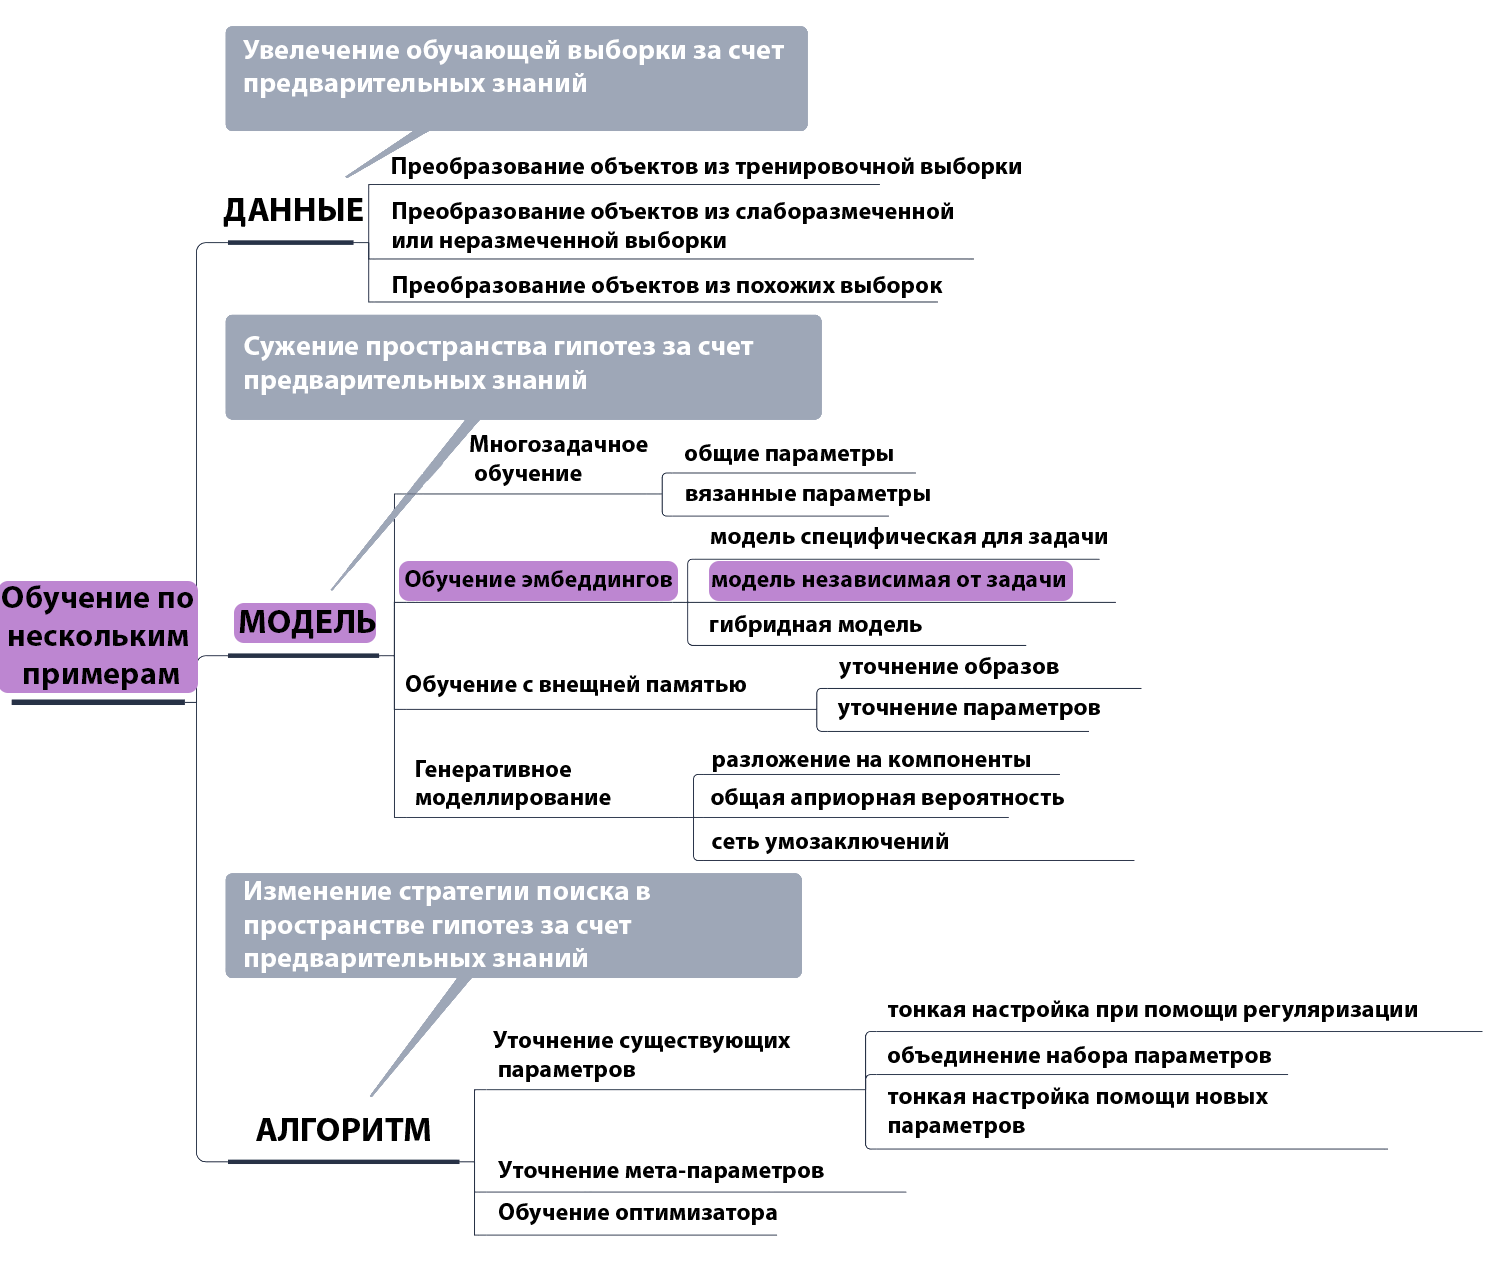
\includegraphics[width=16cm]{Images/FSL_taxomony_rus_noback.png}
\label{fig:FSL_taxomony_rus_noback}
\end{figure}

Легко заметить, что в прикладных задачах могут быть применены различные комбинации подходов или все три одновременно, поскольку они затрагивают разные аспекты обучения. Подробное описание каждого из подходов, изображенных на Рис. \ref{fig:FSL_taxomony_rus_noback} изложено в статье \cite{FSLsurvey}. Тем не менее, поскольку обучение эмбеддингов является неотъемлемой частью данного исследования, ниже изложено более подробное описание этого метода.

\newpage
\subsubsection{Обучение эмбеддингов}

\label{subsec:EmbeddingLearning}

    Суть построения эмбеддингов \cite{ReviewConvolutionArchitectureEmbedding} - перевод объектов из начального пространства ${x_i}\in\mathcal{X}\subset\mathbb{R}^n$ в пространство меньшей размерности ${z_i}\in\mathcal{Z}\subset\mathbb{R}^m, m < n$, в котором уже и производить классификацию. Причем $\mathcal{Z}$ должно быть таким, что похожие примеры должны быть близки друг к другу, а различные - удалены.

    Одним из наиболее простых методов построения сети эмбеддингов является использование части классификатора: сначала строится сеть, классифицирующая на большое число классов, а после удаляется последний слой (слой вывода), оставшаяся часть и есть генератор эмбеддингов (Рис. \ref{fig:embed_from_mlp}).

\begin{figure}[!h]
\caption{Построение генератора эмбеддингов с помощью классификатора}
\centering
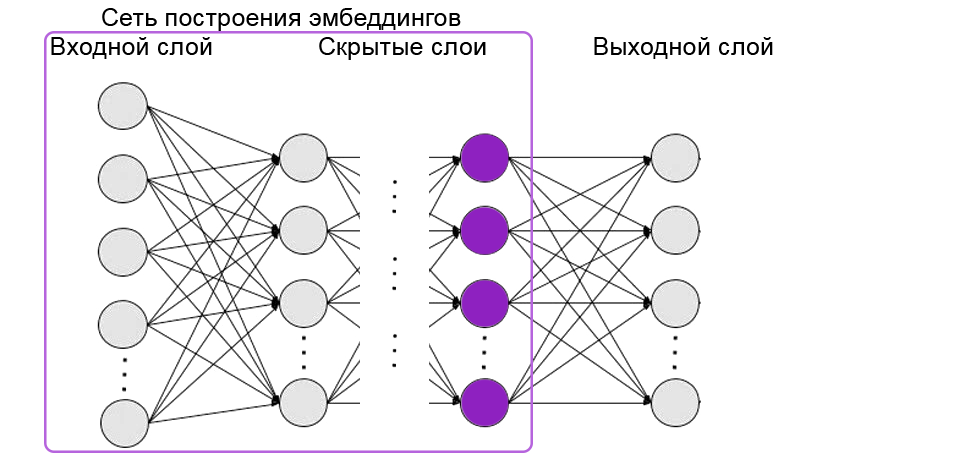
\includegraphics[width=16cm]{Images/embed_from_mlp.png}
\label{fig:embed_from_mlp}
\end{figure}


    Основные компоненты обучения эмбеддингов: функция $f$, переводящая тестовый пример $x_{\text {test }} \in D_{\text {test }}$ в пространство эмбеддингов $\mathcal{Z}$, функция $g$, переводящая объекты из тренировочного датасета $x_i \in D_{\text {train }}$ в $\mathcal{Z}$, функция схожести (расстояния) $s(x_i, x_j)$. Обычно функции $f$ и $g$ совпадают.

    По тому, как меняются параметры функций $f$ и $g$ от задачи к задаче выделяют три метода построения эмбеддингов: индивидуальный для каждой задачи (task-specific), независимый (task-invariant) и гибридный.

\begin{itemize}
    \item \textbf{Task-specific (Специфическая для каждой задачи)} \cite{ReviewEmbedInformationLens}. Обучение проводится только на объектах из обучающей выборки для конкретной задачи. 
    \item \textbf{Task-invariant (Модель, независящая от задачи)} \cite{ReviewEmbedObjectClassification, ReviewSiameseNeuralNetworks} Рис. \ref{fig:FSL_Embedding_general_rus_noback}. Обучение проводится на большой обучающей выборке, а после обученная модель применяется без переобучения для специфической задачи.
    \label{pos:TaskInvariant}
    \item \textbf{Гибридная модель} \cite{ReviewEmbedFeedForward} Рис. \ref{fig:FSL_Embedding_hybrid_rus_noback}. Гибридная модель объединяет в себе предыдущие два подхода: эмбеддинги, полученные при использовании независимой модели, используются как параметр для построения эмбеддингов для конкретной задачи.
\end{itemize}

\begin{figure}[h!]
\caption{Независимая модель построения эмбеддингов}
\centering
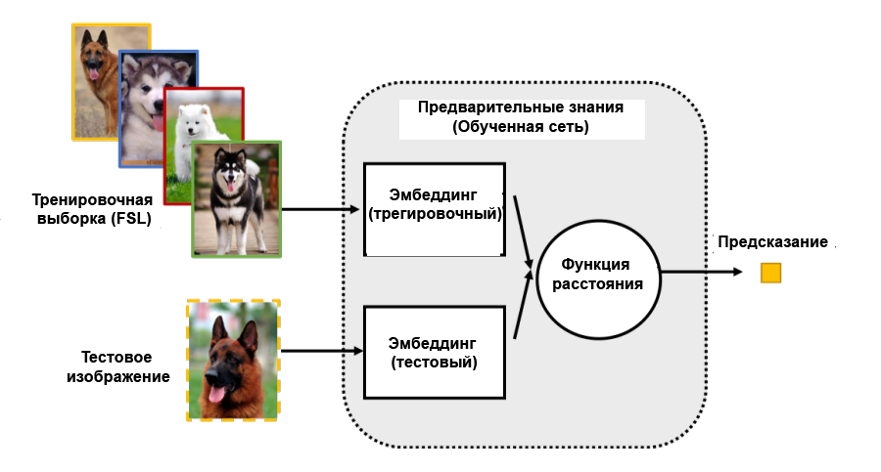
\includegraphics[width=16cm]{Images/FSL_Embedding_general_rus_noback.png}
\label{fig:FSL_Embedding_general_rus_noback}
\end{figure}

\begin{figure}[h!]
\caption{Гибридная модель построения эмбеддингов}
\centering
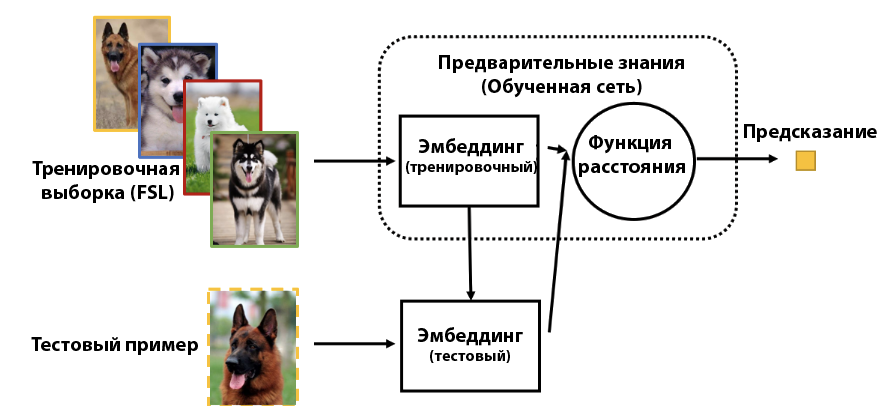
\includegraphics[width=16cm]{Images/FSL_Embedding_hybrid_rus_noback.png}
\label{fig:FSL_Embedding_hybrid_rus_noback}
\end{figure} % Обзор существующих решений
\section{Постановка задачи}
\label{sec:Chapter2} \index{Chapter2}

Рассмотрим методы основанные на построении эмбеддингов. Эффективность таких сетей применительно к формированию пространства эмбеддингов существенно зависит от выбора функции потерь, поэтому проведем сравнительное исследование этих функций потерь. Для проведения такого исследования предлагается следующая постановка задачи: дан некоторый набор данных для обучения, необходимо построить сеть для генерации эмбеддингов и обучить ее с применением нескольких функций потерь. Требуется провести сравнительное исследование полученных пространств эмбеддингов с учетом их дальнейшего использования для решения задач FSL.

Этапы решения задачи:
\begin{itemize}
    \item Провести обзор наиболее популярных функций потерь в области FSL, а также реалиовать их.
    \item Выбрать метод оценки качества пространств эмбеддингов.
    \item Выбрать задачу для проведения эксперимента и модель нейронной сети.
    \item Провести сравнительный анализ пространств эмбеддингов, полученных с использованием выбранных функций потерь.
\end{itemize} % Постановка задачи
\section{Предлагаемое решение}
\label{sec:Chapter3} \index{Chapter3}


\subsection{Функции потерь}
\label{sec:LossFunctions}
    Теперь рассмотрим специфические для задачи построения эмбеддингов функции потерь \cite{weng2021contrastive}, предполагаемо улучшающие кластеризацию.

\subsubsection{Contrastive loss}

Contrastive loss \cite{LossContrstive} для каждой пары объектов $\left(x_i, x_j\right)$ минимизирует расстояние эмбеддингов, если они из одного класса, и максимизирует, если они из разных классов:


$\begin{aligned} \mathcal{L}_{\text {cont }}\left(\mathbf{x}_i, \mathbf{x}_j, \theta\right) = & \mathbb{1}\left[y_i=y_j\right]\left\|f_\theta\left(\mathbf{x}_i\right)-f_\theta\left(\mathbf{x}_j\right)\right\|_2^2+ \\ & \mathbb{1}\left[y_i \neq y_j\right] \max \left(0, \epsilon-\left\|f_\theta\left(\mathbf{x}_i\right)-f_\theta\left(\mathbf{x}_j\right)\right\|_2\right)^2\end{aligned}$


Где $\epsilon$ это гиперпараметр, определяющий минимальное расстояние между объектами разных классов.

\subsubsection{Triplet loss}
\begin{figure}[h!]
\caption{Схема работы Triplet Loss}
\centering
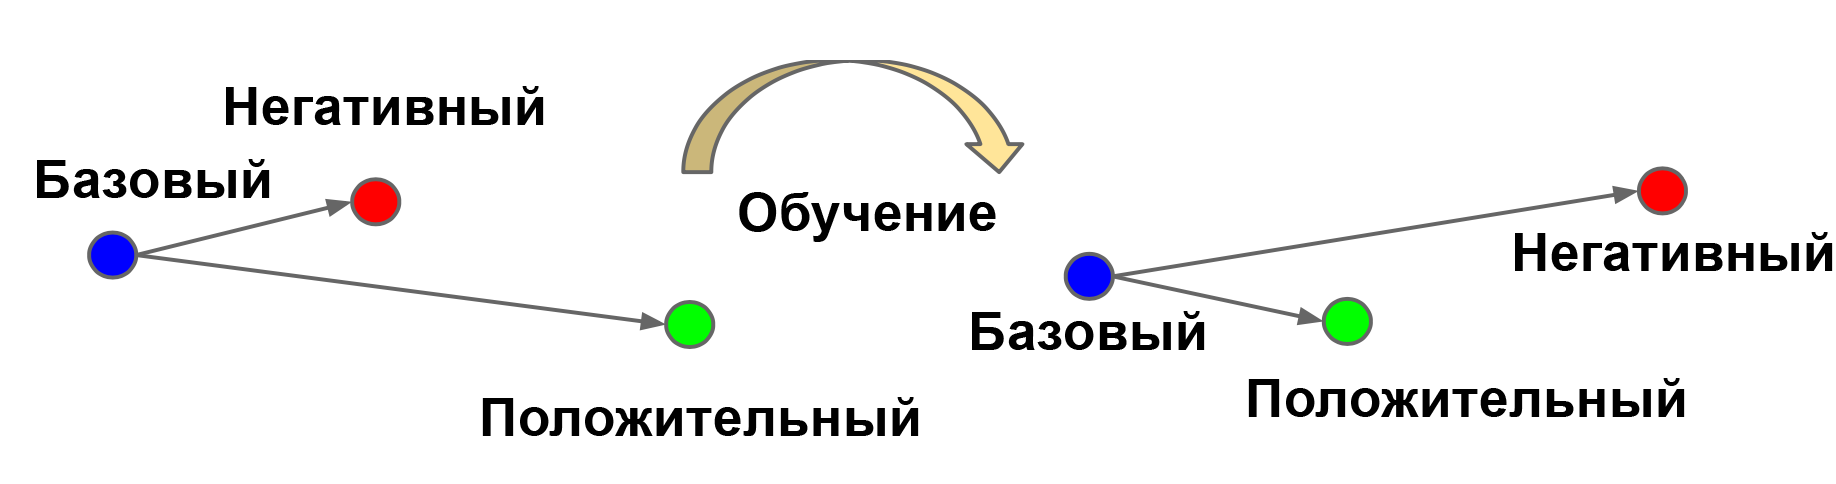
\includegraphics[width=16cm]{Images/triplet_loss_rus_noback.png}
\label{fig:triplet_loss_rus_noback}
\end{figure}

\label{img:TripletLoss}
    Triplet Loss \cite{LossTriplet} развивает идею Contrastive loss, но расчет идет сразу по трем объектам: базовый пример $\mathbf{x}$, положительный  пример (того же класса, что и базовый) $\mathbf{x}^{+}$ и один негативный пример (другого класса) $\mathbf{x}^{-}$. Triplet loss одновременно увеличивает расстояние между базовым и негативным объектами и уменьшает расстояние между базовым и положительным. (Рис \ref{fig:triplet_loss_rus_noback}):

\begin{center}
$$
\mathcal{L}_{\text {triplet }}\left(\mathbf{x}, \mathbf{x}^{+}, \mathbf{x}^{-}\right)=\sum_{\mathbf{x} \in \mathcal{X}} \max \left(0,\left\|f(\mathbf{x})-f\left(\mathbf{x}^{+}\right)\right\|_2^2-\left\|f(\mathbf{x})-f\left(\mathbf{x}^{-}\right)\right\|_2^2+\epsilon\right)
$$
\end{center}

\subsubsection{Lifted Structured loss}
Lifted Structured loss \cite{LossLifted} работает по тому же принципу, что и Triplet loss, однако он использует все пары объектов внутри одного тренировочного батча (Рис. \ref{fig:lifted_structured_loss_rus_noback}).

\begin{figure}[h!]
\caption{Сравнение функций потерь по выбору объектов}
\centering
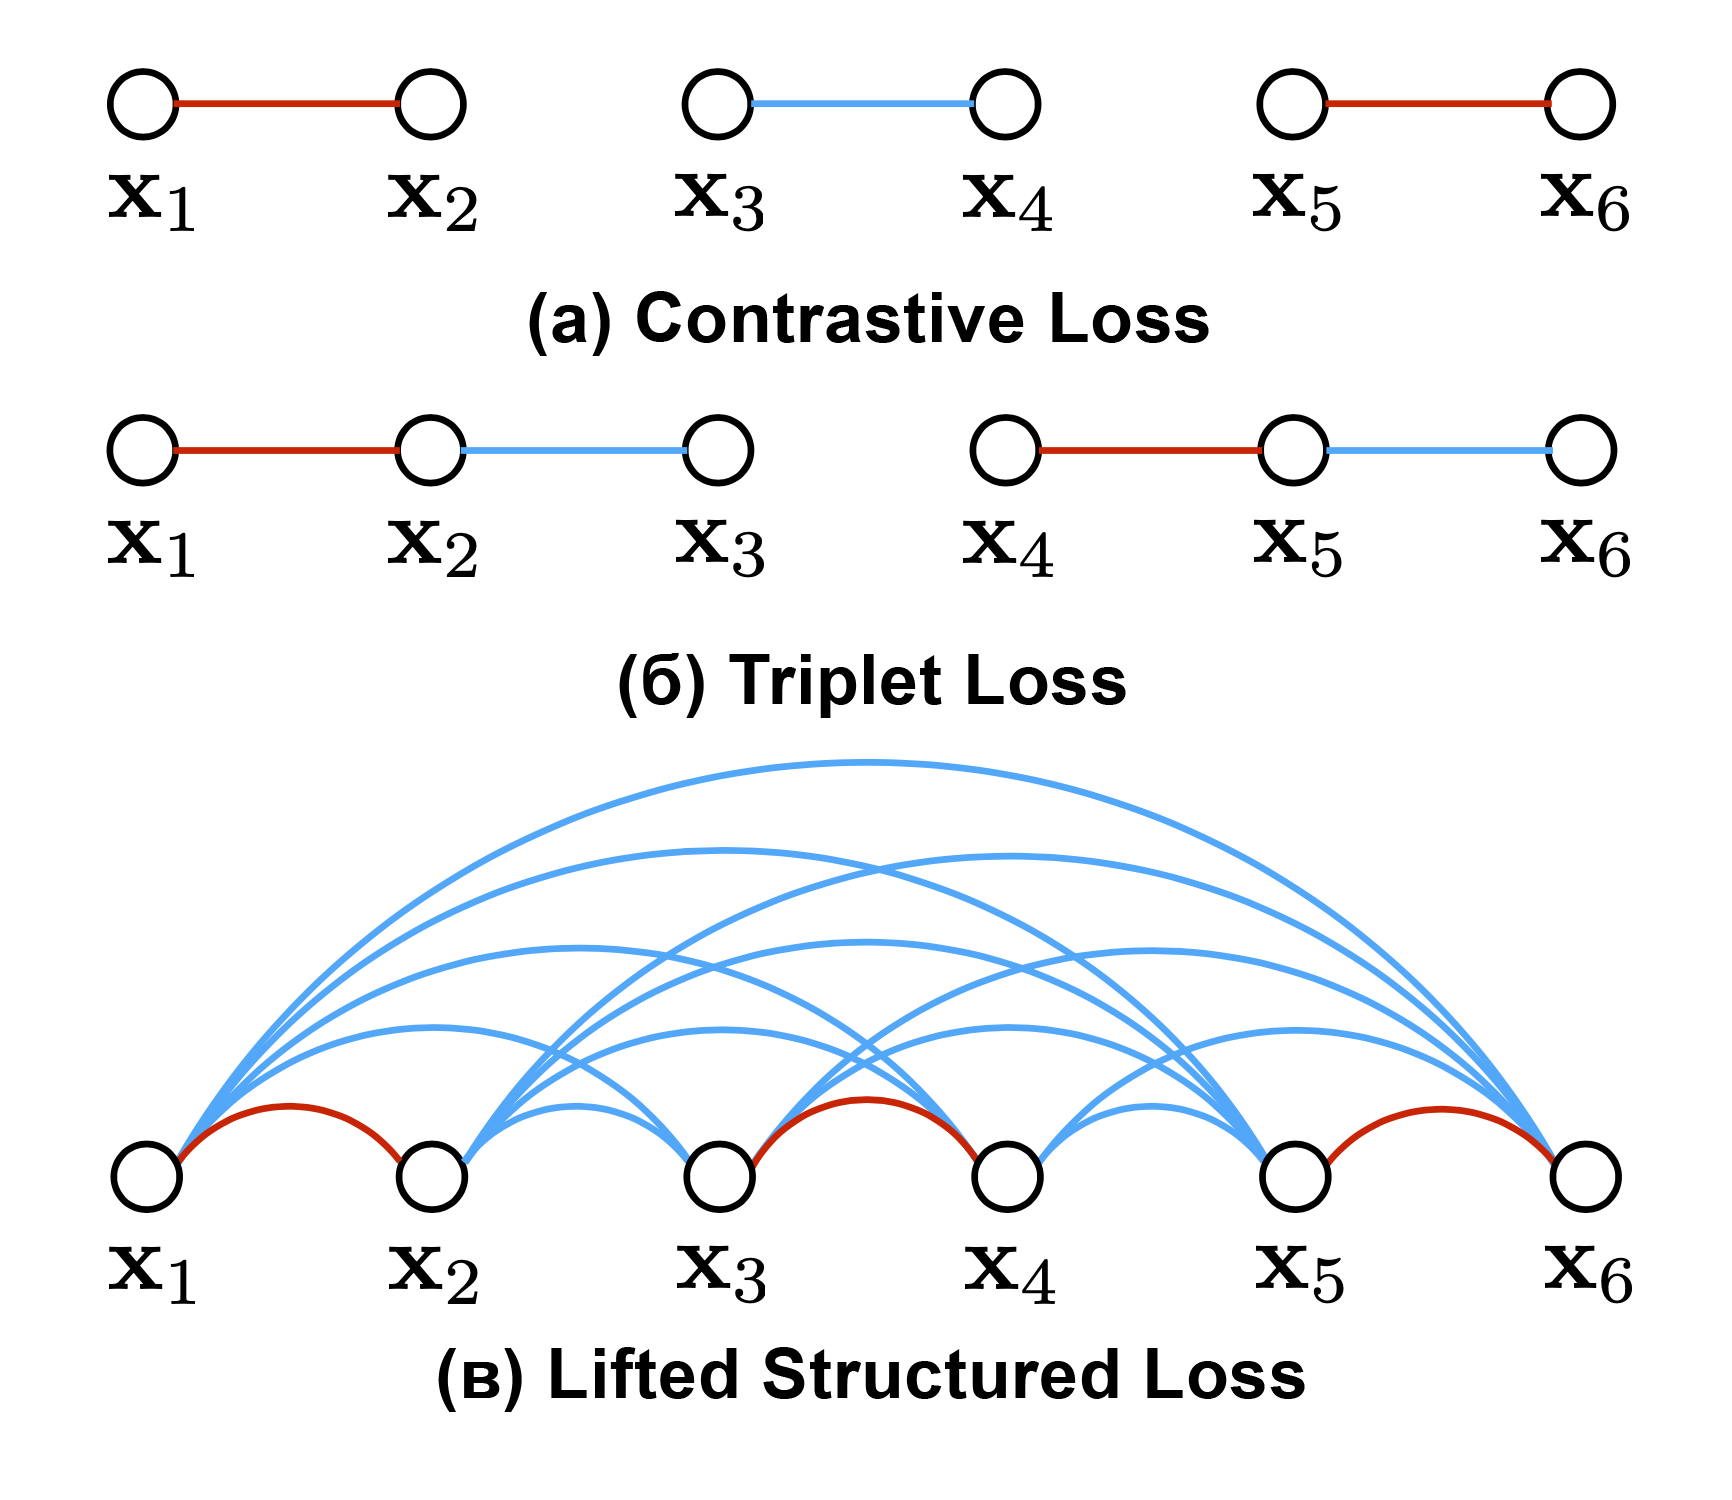
\includegraphics[width=16cm]{Images/lifted_structured_loss_rus_noback.png}
\label{fig:lifted_structured_loss_rus_noback}
\end{figure}


Пусть $D_{i j}=\left|f\left(\mathbf{x}_i\right)-f\left(\mathbf{x}_j\right)\right|_2$, $\mathcal{P}$ - набор положительных примеров, $\mathcal{N}$ - набор отрицательных примеров, тогда:

$$
\begin{aligned}
\mathcal{L}_{\text {struct }} & =\frac{1}{2|\mathcal{P}|} \sum_{(i, j) \in \mathcal{P}} \max \left(0, \mathcal{L}_{\text {struct }}^{(i j)}\right)^2 \\
\text { where } \mathcal{L}_{\text {struct }}^{(i j)} & =D_{i j}+\max \left(\max _{(i, k) \in \mathcal{N}} \epsilon-D_{i k}, \max _{(j, l) \in \mathcal{N}} \epsilon-D_{j l}\right)
\end{aligned}
$$

Правая часть в $\mathcal{L}_{\text {struct }}^{(i j)}$ призвана искать сложные негативные примеры (наиближайшие отрицательные примеры к базовому). Однако это функция ступенчатая, что может вызвать проблемы во время обучения, поэтому используют её сглаженную версию:

$$
\mathcal{L}_{\text {struct }}^{(i j)}=D_{i j}+\log \left(\sum_{(i, k) \in \mathcal{N}} \exp \left(\epsilon-D_{i k}\right)+\sum_{(j, l) \in \mathcal{N}} \exp \left(\epsilon-D_{j l}\right)\right)
$$

\subsubsection{N-pair loss}

N-pair loss \cite{LossNpair} -  это обобщение triplet loss, использующее не один, а несколько ($N-1$) негативных примеров. Таким образом, выбирается базовый пример, один положительный и ($N-1$) негативных примеров.
$$
\begin{aligned}
\mathcal{L}_{\mathrm{N}-\mathrm{pair}}&\left(\mathbf{x}, \mathbf{x}^{+},\left\{\mathbf{x}_i^{-}\right\})_{i=1}^{N-1}\right)  =\log \left(1+\sum_{i=1}^{N-1} \exp \left(f(\mathbf{x})^{\top} f\left(\mathbf{x}_i^{-}\right)-f(\mathbf{x})^{\top} f\left(\mathbf{x}^{+}\right)\right)\right) \\
& =-\log \frac{\exp \left(f(\mathbf{x})^{\top} f\left(\mathbf{x}^{+}\right)\right)}{\exp \left(f(\mathbf{x})^{\top} f\left(\mathbf{x}^{+}\right)\right)+\sum_{i=1}^{N-1} \exp \left(f(\mathbf{x})^{\top} f\left(\mathbf{x}_i^{-}\right)\right)}
\end{aligned}
$$

\begin{figure}[h!]
\caption{Формирование пакета для N-pair loss}
\centering
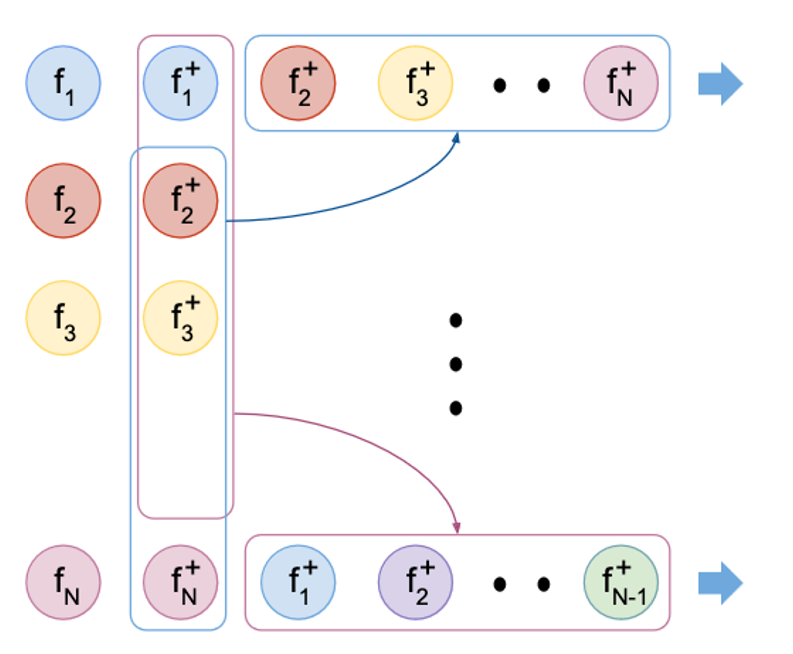
\includegraphics[width=12cm]{Images/N_pair_batch.png}
\label{fig:N_pair_batch}
\end{figure}

\subsection{Кластеризация}
    Как следует из цели подхода, основанного на построении эмбеддингов, исходные данные должны быть разделимы в новом пространстве. Это особенно важно для экстремальных случаев FSL: обучение по одному примеру (One Shot Learning или OSL) или обучение без примеров (Zero Shot Learning или ZSL). На Рис. \ref{fig:ClusteringGoodPoor} точками изображены экземпляры двух синтетических классов. Если кластеры достаточно удалены друг от друга, то нам не важно какие точки выбрать (какие примеры нам попадутся в обучающей выборке) для построения разделяющей гиперплоскости (в данном случае прямой), а если кластеры близки или вообще пересекаются, то качество разделяющей гиперплоскости будет зависеть от полученных примеров. Следовательно для оценки свойств полученного пространства будем вычислять метрики, характеризующие свойства  кластеризации данных.

    \begin{figure}[!ht]
      \begin{center}
          
      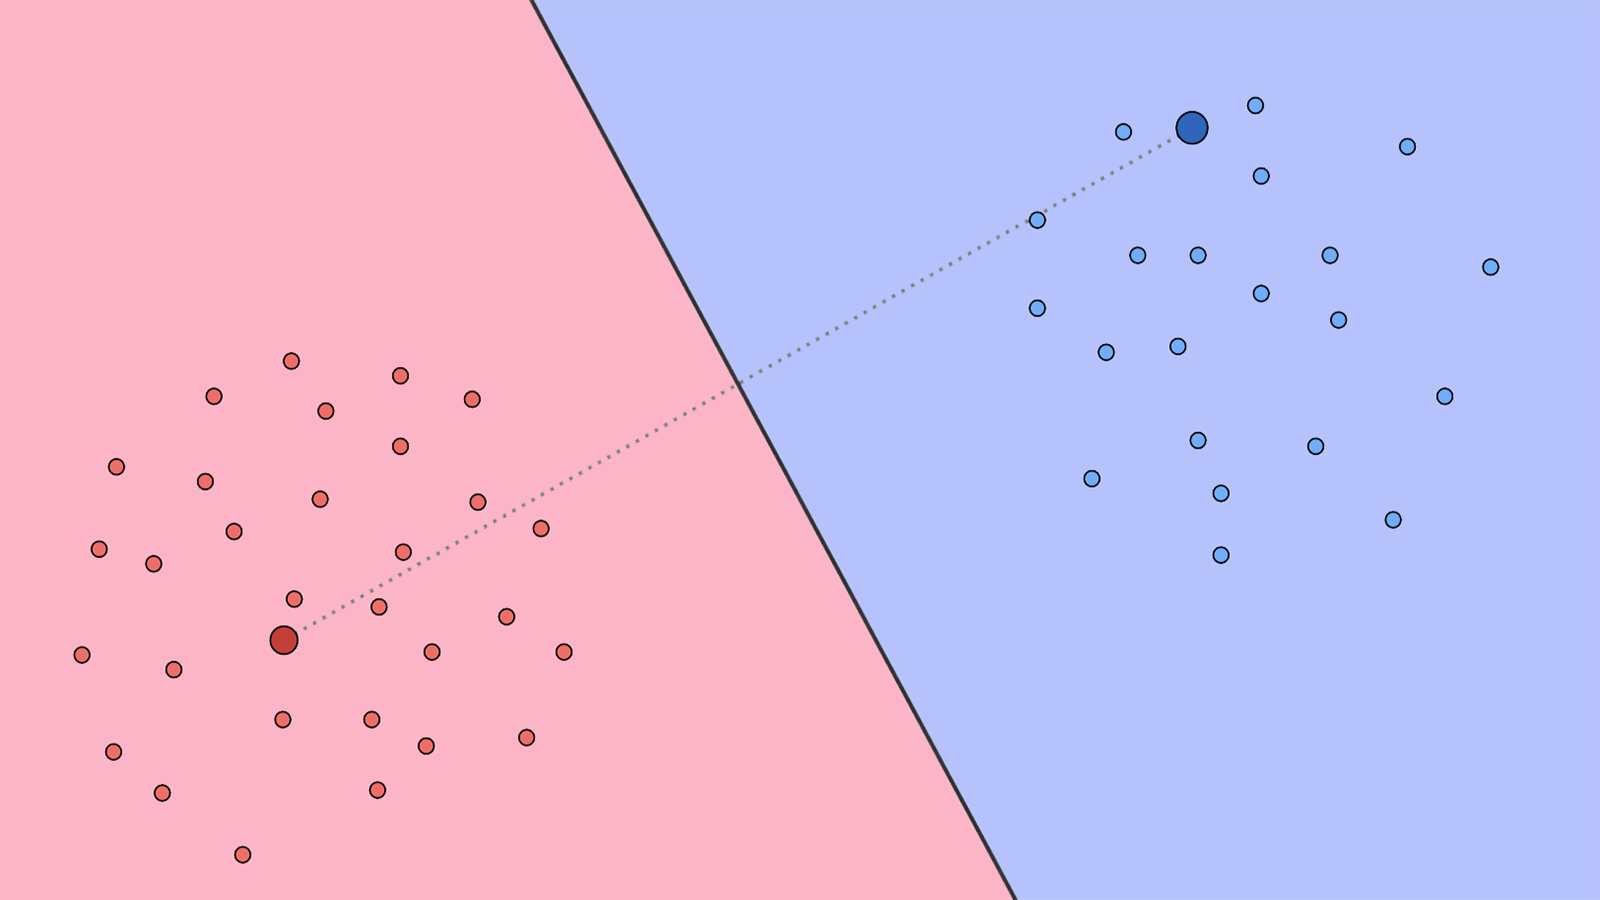
\includegraphics[width=10cm]{Images/good_clustering.png}
      \caption*{(a)}
      
      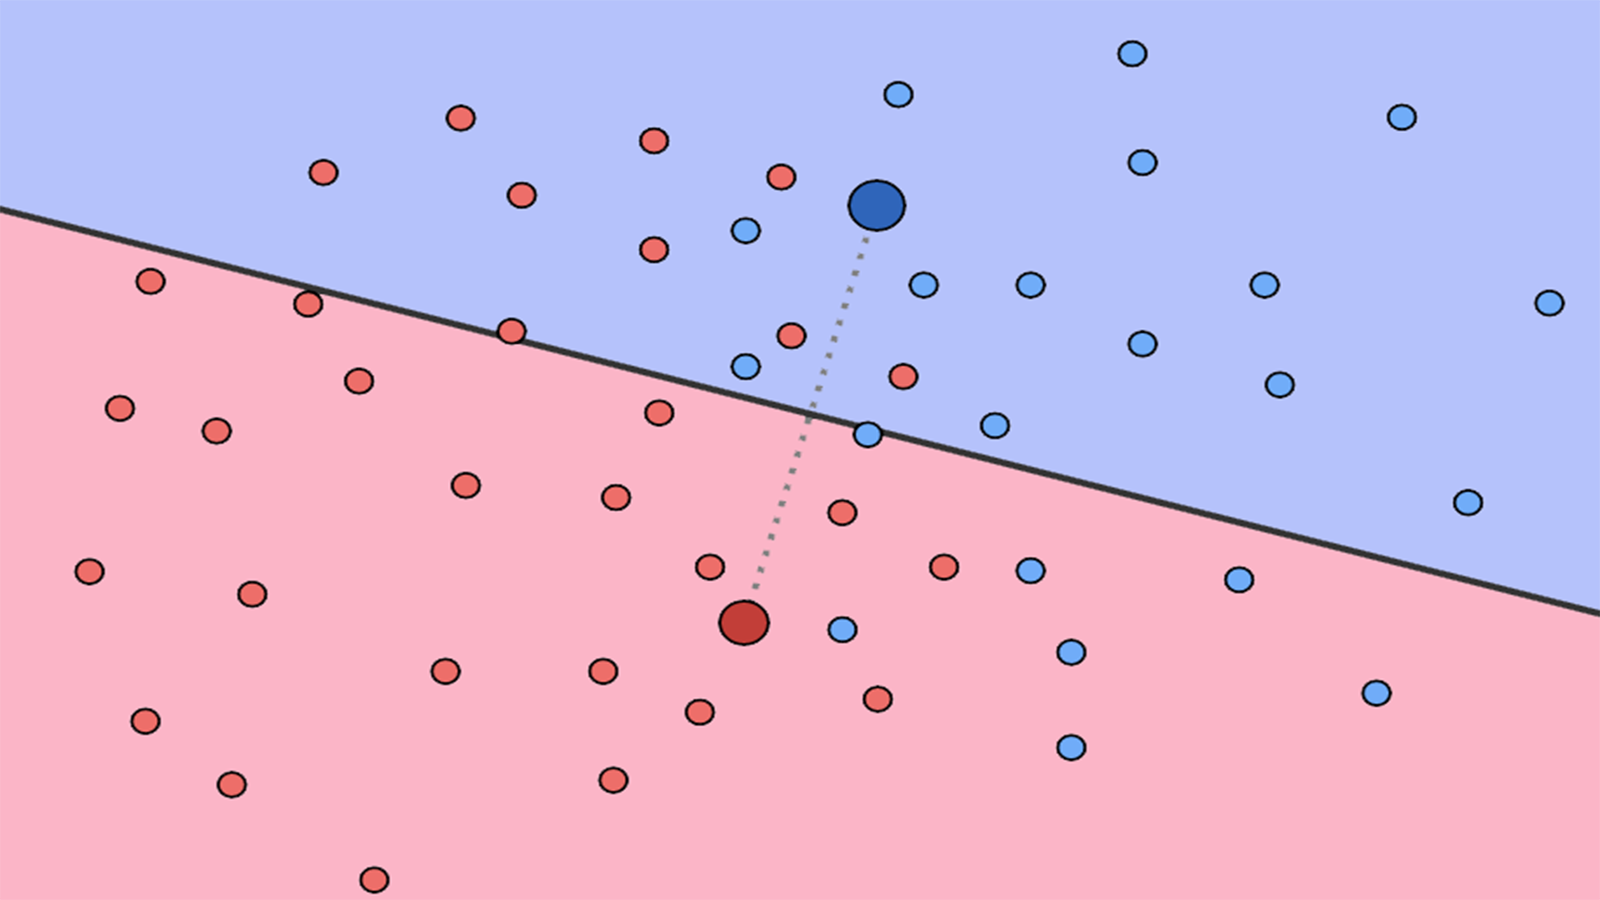
\includegraphics[width=10cm]{Images/poor_clustering.png}
      \caption*{(b)}      
      
      \end{center}
    \caption{Примеры хорошей (a) и плохой (b) класетризации}
    \label{fig:ClusteringGoodPoor}
    \end{figure}
    
\subsubsection{Оценка качества}
\label{subsec:ClusteringQuality}
    Для определения качества кластеризации вводятся следующие функции \cite{EmbedMetaFSL}:
    \begin{itemize}
        \item Отношение внутриклассовой к межклассовой дисперсии (intra-class to inter-class variance ratio): 
        \begin{center}
            
        \Large
        $R_{FC}=\frac{\sigma_{\text {within }}^2}{\sigma_{\text {between }}^2}=\frac{\frac{\sum_{i, j}\left\|\phi_{i, j}-\mu_i\right\|_2^2}{N}}{\frac{\sum_i\left\|\mu_i-\mu\right\|_2^2}{C}}=\frac{C}{N} \frac{\sum_{i, j}\left\|\phi_{i, j}-\mu_i\right\|_2^2}{\sum_i\left\|\mu_i-\mu\right\|_2^2}$,
        
        \end{center}
        \normalsize

        где $C$ - количество классов, $N$ - количество объектов в классе,  $\phi_{i, j}$ - эмбеддинг $j$-ого объекта в $i$-ом классе, $\mu_i$ - среднее эмбеддингов $i$-ого класса, $\mu$ - среднее эмбеддингов всех классов.
        Чем меньше значение полученного выражения, тем лучше кластеризация.

        \item Ограничение разброса гиперплоскостей: Пусть $x_1, x_2$ - объекта одного класса, $y_1, y_2$ - объекты другого класса, $f_\theta\left(x\right)$ - эмбеддинг объекта $x$, тогда выражение $f_\theta\left(x_1\right)-f_\theta\left(y_1\right)$ показывает направление разделяющей гиперплоскости с наибольшим зазором. Следующее выражение показывает насколько разные гиперплоскости можно построить, выбирая различные пары объектов из двух классов: 
        
        \begin{center}

        \Large
        
        $\begin{aligned} R_{HV} & \left(f_\theta\left(x_1\right), f_\theta\left(x_2\right), f_\theta\left(y_1\right), f_\theta\left(y_2\right)\right) \\ & =\frac{\left\|\left(f_\theta\left(x_1\right)-f_\theta\left(y_1\right)\right)-\left(f_\theta\left(x_2\right)-f_\theta\left(y_2\right)\right)\right\|_2}{\|\left(f_\theta\left(x_1\right)-f_\theta\left(y_1\right)\left\|_2+\right\| f_\theta\left(x_2\right)-f_\theta\left(y_2\right) \|_2\right.} .\end{aligned}$
        
        \end{center}
        \normalsize
        Как и в первом случае чем меньше значение $R_{H V}$, тем лучше кластеризация.
        
    \end{itemize}

\subsection{Тестовая задача}
Для проведения экспериментов выбрана задача распознавания ключевых слов (Keyword Spotting) на пример набора данных Google Speech V2 \cite{GoogleSpeechDataset}. Датасет представляет собой набор из 105,829 примеров для 35 различных английских слов. Каждый пример представляет собой аудио файл формата WAV, длительностью не более одной секунды. В записи участвовали 2618 людей. Также, помимо примеров самих слов, датасет предоставляет несколько файлов с фоновым шумом. 

На вход нейронной сети подается представление аудио файла в виде мел спектрограммы: в отличие от обыной спектрограммы используется нелинейная шкала частот, отображающая воприятие звука человеком. Так, для более низких частот получается больше делений (мелов), чем для высоких. В итоге, в качеств входа модели выступает двумерный массив, для которого естественно использовать сверточные нейронные сети.

\subsection{Тестовая модель}
В качестве базовой модели выбрана модификация светрочной нейронной сети под названием Depthwise Separable Convolution Neural Network (DS-CNN). В статье \cite{KeywordSpottingMicrocontrollers} проводилось сравнение различных моделей нейронных сетей на датасете Google Speech V1, в ходе которого DS-CNN показала наилучшую точность при сопоставимом числе операций. Общая структура DS-CNN модели представлена на Рис. \ref{fig:DS_CNN_model}. В ходе экспериметнов использовался вариант DS-CNN, включающий в себя 4 блока DS-Conv, каждый по 64 карты признака. Размерность пространства эмбеддингов (количество нейрнов после слоя Average Pool) также 64.

\begin{figure}[h!]
\caption{Структура DS-CNN}
\centering
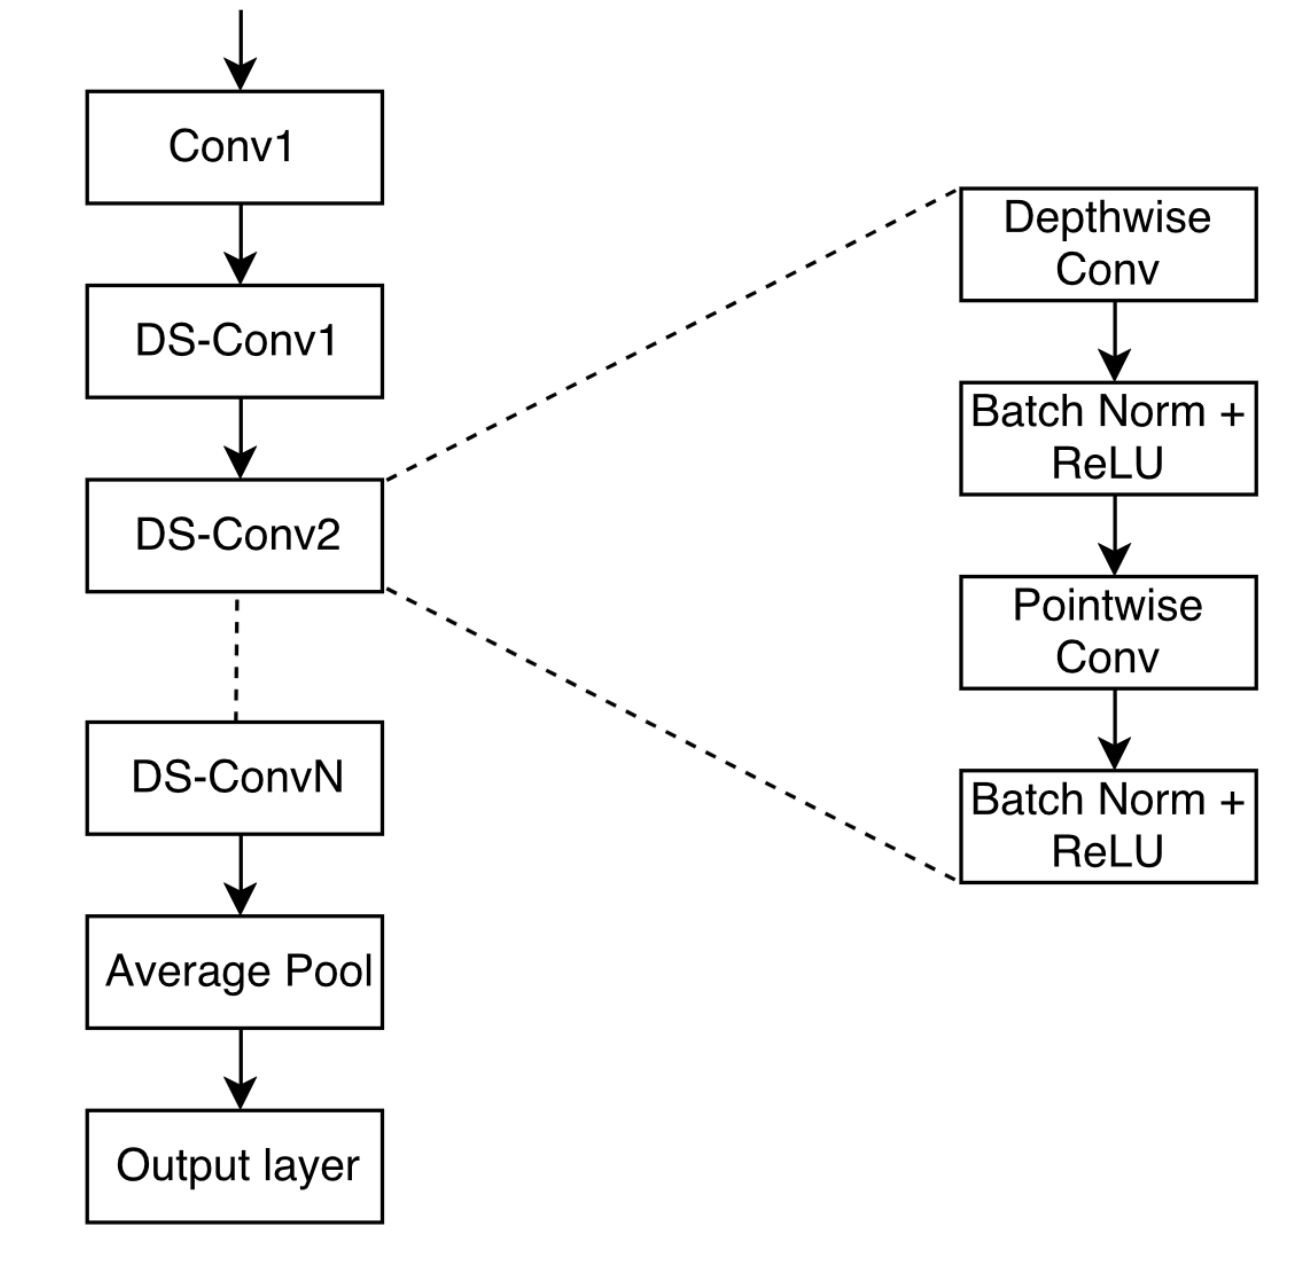
\includegraphics[width=16cm]{Images/DS_CNN_model.png}
\label{fig:DS_CNN_model}
\end{figure} % Один или несколько пунктов, посвященных детальному описанию тех решений, которые Вы разработали/реализовали
\section{Программная реализация}
\label{sec:Chapter4} \index{Chapter4}

Для выполнения поставленной задачи использовался язык Python 3. Основной библиотекой для построения и обучения моделей стал PyTorch. В ходе работы были реализованы следующие компоненты:
\begin{itemize}
    \item Функции потерь
    \begin{itemize}
        \item Triplet Loss
        \item N-pair loss
        \item Lifted-Structured Loss
    \end{itemize}
    \item Функции для формирования пакетов (батчей) для каждой из перечисленных функций потерь
    \item Метрики качества кластеризации
    \begin{itemize}
        \item FC - feature clustering
        \item HC - hyperplane variation
    \end{itemize}
\end{itemize}

Эксперименты проводились на платформе Jupyter Notebook на локальной машине с использованием видеокарты Nvidia RTX 3060 TI 8GB. % Программная реализация
\section{Эксперименты}
\label{sec:Chapter5} \index{Chapter5}

\par
Для оценки качества кластеризации в рамках задач FSL датасет Google Speech V2 разделим на две непересекающиеся части (разделение имеет случайный характер): 
\begin{enumerate}
    \item Первый набор используется для обучения и включает в себя все примеры следующих 20 слов: \textit{ \{'four', 'on', 'nine', 'dog', 'marvin', 'eight', 'five', 'down', 'three', 'right', 'yes', 'backward', 'tree', 'zero', 'off', 'cat', 'up', 'bed', 'six', 'two'\}}, что в сумме дает 65768 примеров.
    \item Второй набор используется для тестирования и включает в себя все примеры оставшихся 15 слов: \textit{\{'follow', 'house', 'one', 'left', 'sheila', 'happy', 'learn', 'forward', 'stop', 'visual', 'go', 'bird', 'no', 'seven', 'wow'\}}, что в сумме дает 40061 пример.
\end{enumerate}
Для обучения первый набор делится на тренировочную (70\% или 46037 примеров) и валидационную (30\% или 19731 пример) выборки. Использовались следующие параметры обучения:

\begin{itemize}
    \item Оптимизатор - Adam.
    \item Размер батча - 100.
    \item Количество эпох - 25.
    \item Learning rate - $1 * 10^{-4}$.
\end{itemize}

\par
В качестве точки отсчета выбран классификатор, обученный с использованием функцией потерь кросс-энтропия. После обучения классификатора, для получения вектора эмбеддинга использовался предпоследний слой - 'Average Pool' Рис.\ref{fig:DS_CNN_model}. Для обучения с использованием остальных функций потерь использовалась та же модель DS-CNN сразу без 'Output layer'. Таким образом, получается одинаковая сложность и структура модели как для базового классификатора, так и для специальных функций потерь.

\par
В процессе обучения проводились промежуточные вычисления метрик FC и HV как на валидационной выборке, так и на тестовой. Для этого брались по 10 случайных батчей (1000 примеров) отдельно для каждой выборки. Изменение значений метрик в процессе обучения изображены на следующих графиках: FC Рис. \ref{fig:FC_aggregate}, HV Рис. \ref{fig:HV_aggregate}. Результаты обученных моделей представлены в таблице \ref{table:1}.

\begin{table}[!h]
\centering
\begin{tabular}{|p{3.5 cm}|p{1.5 cm}|p{1.5 cm}|p{1.2 cm}|p{1.2 cm}|p{1.8 cm}|p{1.8 cm}|}
\hline
Функция потерь    & FC Train & HV Train & FC Test & HV Test  \\ \hline
Cross-Entropy     & 0.70     & 0.50     & 1.51    & 0.57     \\ \hline
Triplet           & 0.44     & 0.45     & 1.22    & 0.58     \\ \hline
Lifted Structured & 0.32     & 0.42     & 0.93    & 0.54     \\ \hline
N-pair            & 0.55     & 0.48     & 1.23    & 0.58     \\ \hline         
\end{tabular}
\caption{Результаты экспериментов}
\label{table:1}
\end{table}

Как видно из таблицы \ref{table:1} наилучшие результаты по метрикам FC и HV с большим отрывом, как на тренировочной, так и на тестовой части, принадлежат функции Lifted Structured Loss.

\begin{figure}[!h]
\caption{Изменение FC в процессе обучения}
\centering
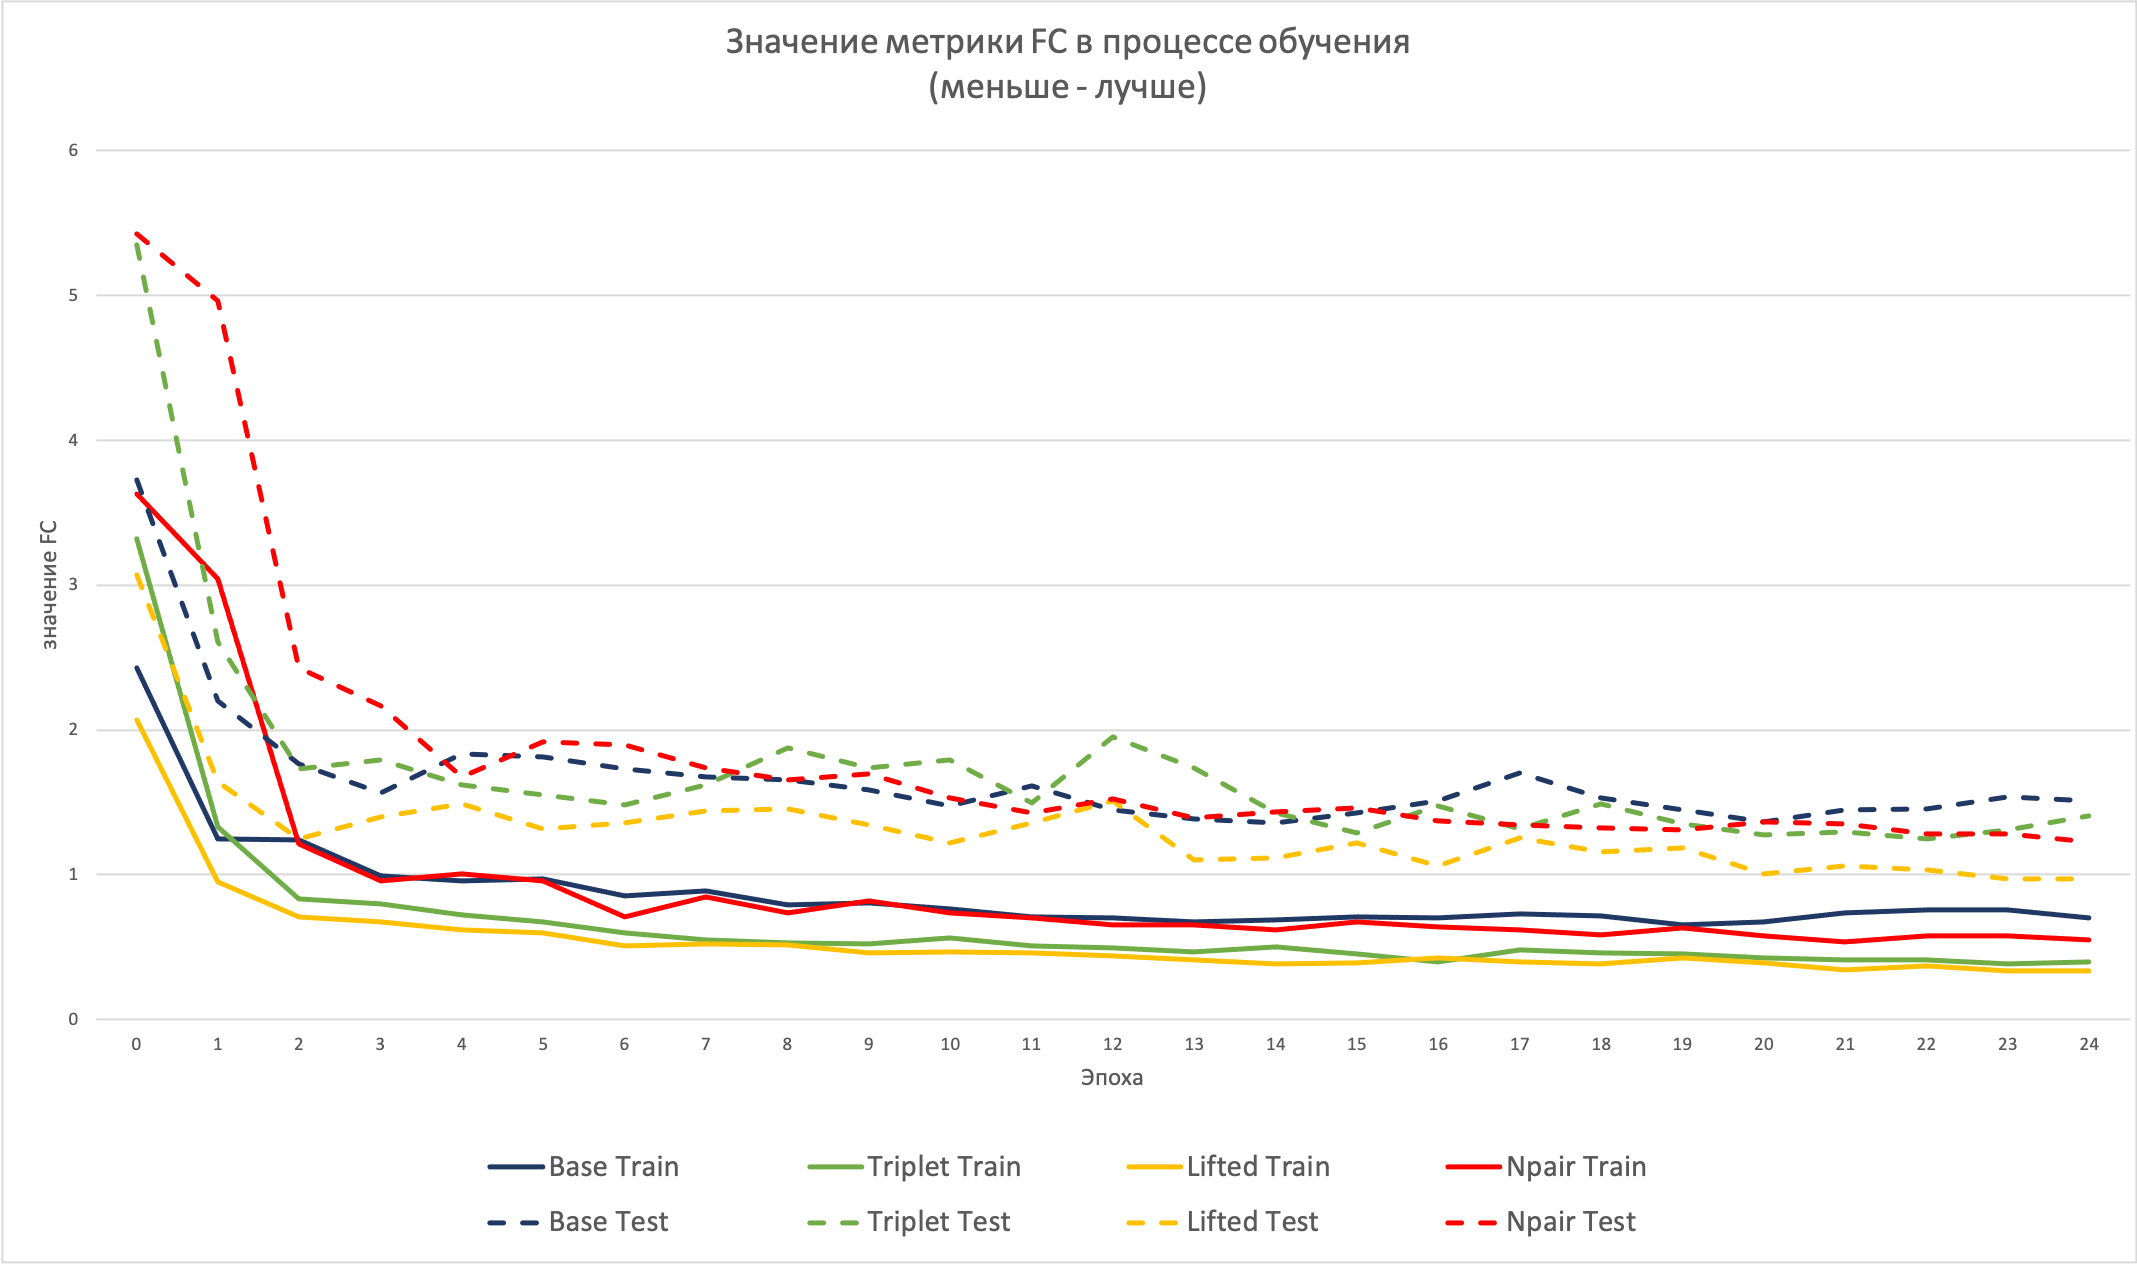
\includegraphics[width=16cm]{Images/FC_aggregate.png}
\label{fig:FC_aggregate}
\end{figure}

\begin{figure}[!h]
\caption{Изменение HV в процессе обучения}
\centering
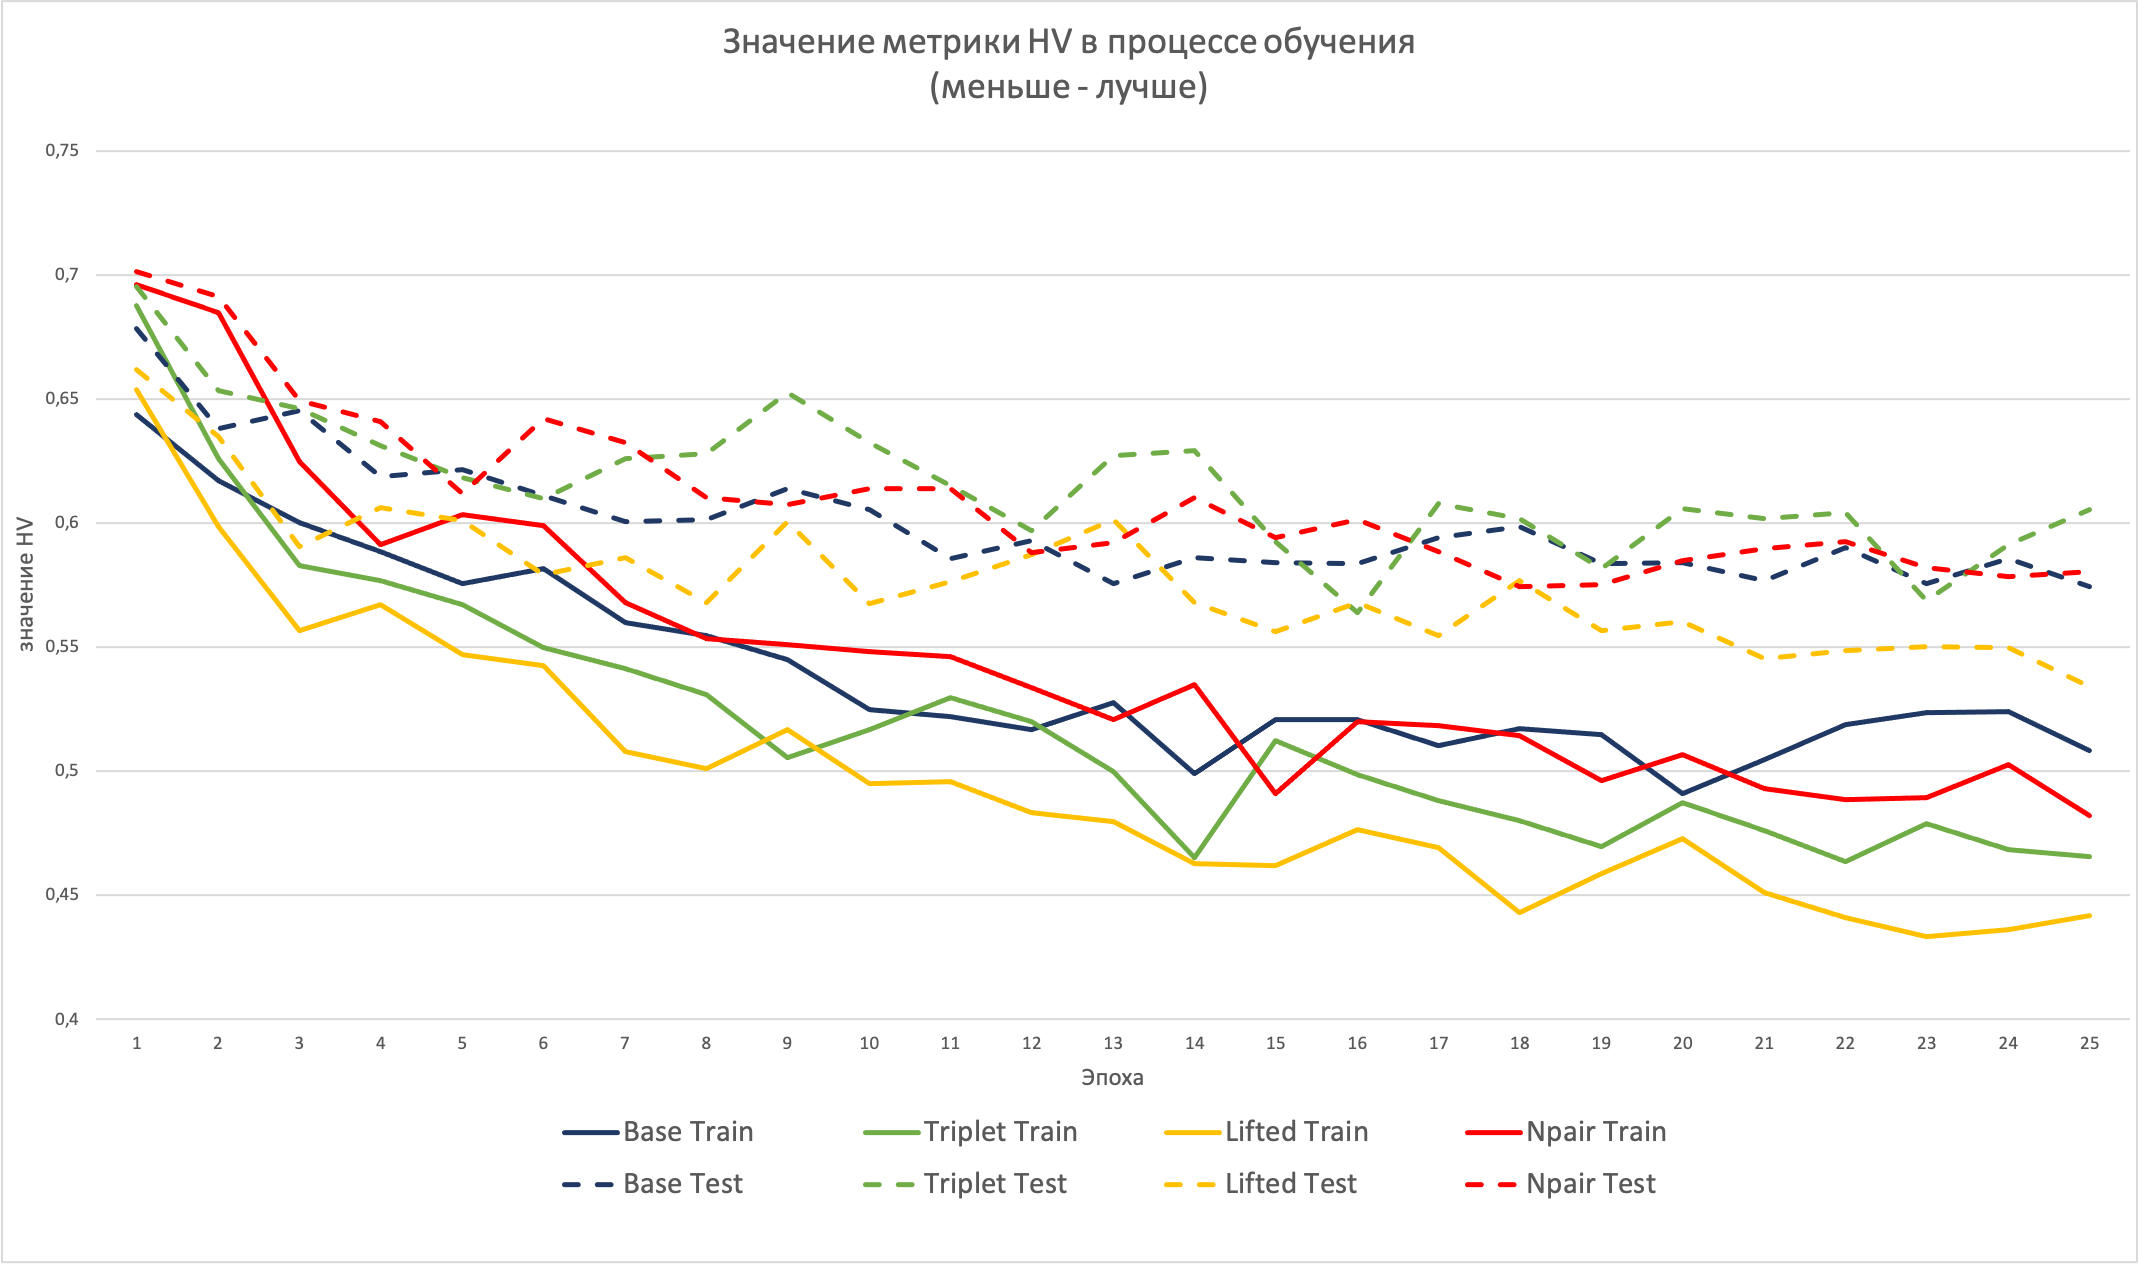
\includegraphics[width=16cm]{Images/HV_aggregate.png}
\label{fig:HV_aggregate}
\end{figure}

\par
Помимо численного подтверждения образования кластеров посредством выбранных метрик, была произведено отображение эмбеддингов в пространство размерности 2 с использованием t-SNE из бибилиотеки scikit-learn. Для проведения сравнения были выбраны по 500 случайных примеров из обучающей и тестовой выборки. На тренировочном наборе Рис.\ref{fig:tsne_train_4} видно, что во всех случаях большую часть кластеров легко выделить, однако базовая модель-классификатор и Lifted Structured Loss показали себя лучше остальных. На тестовом наборе ситуация сильно ухудшается, что ожидаемо по вычисленным ранее метрикам. Тем не менее в случае Lifted Structured Loss получились довольно плотные кластера для слов 'forward' (рыжие точки), 'go' (темно-зеленые), 'wow' (светло-голубые), 'follow' (серо-голубые), 'stop' (блекло-желтыые). Данные отобрадения дополнительно подтвердают формирование кластеров в процессе обучения с использованием описанных функций потерь, а также дает возможность изобразить превосходство использования Lifted Structured Loss.

\newpage


\begin{figure}[!h]
\caption{Применение t-SNE на тренировочном наборе}
\centering
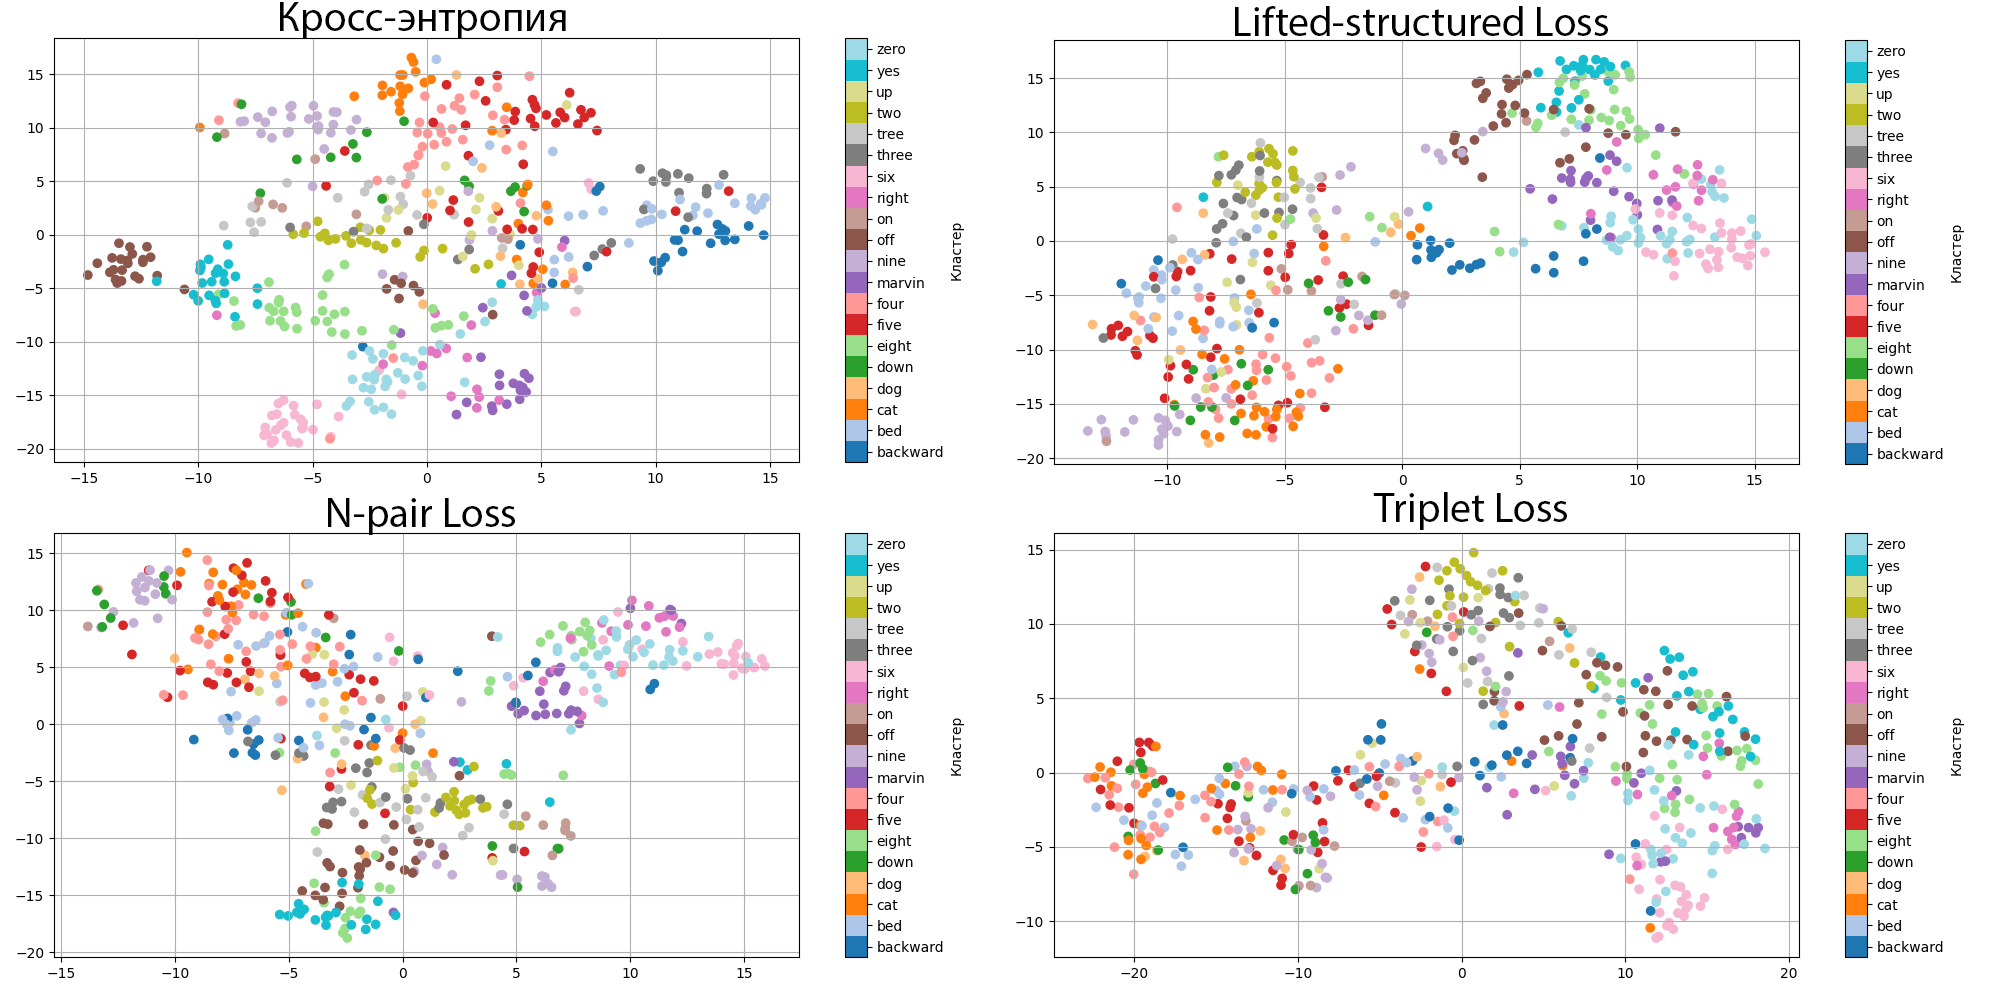
\includegraphics[width=16cm]{Images/tsne_train_4.png}
\label{fig:tsne_train_4}
\end{figure}

\begin{figure}[!h]
\caption{Применение t-SNE на тестовом наборе}
\centering
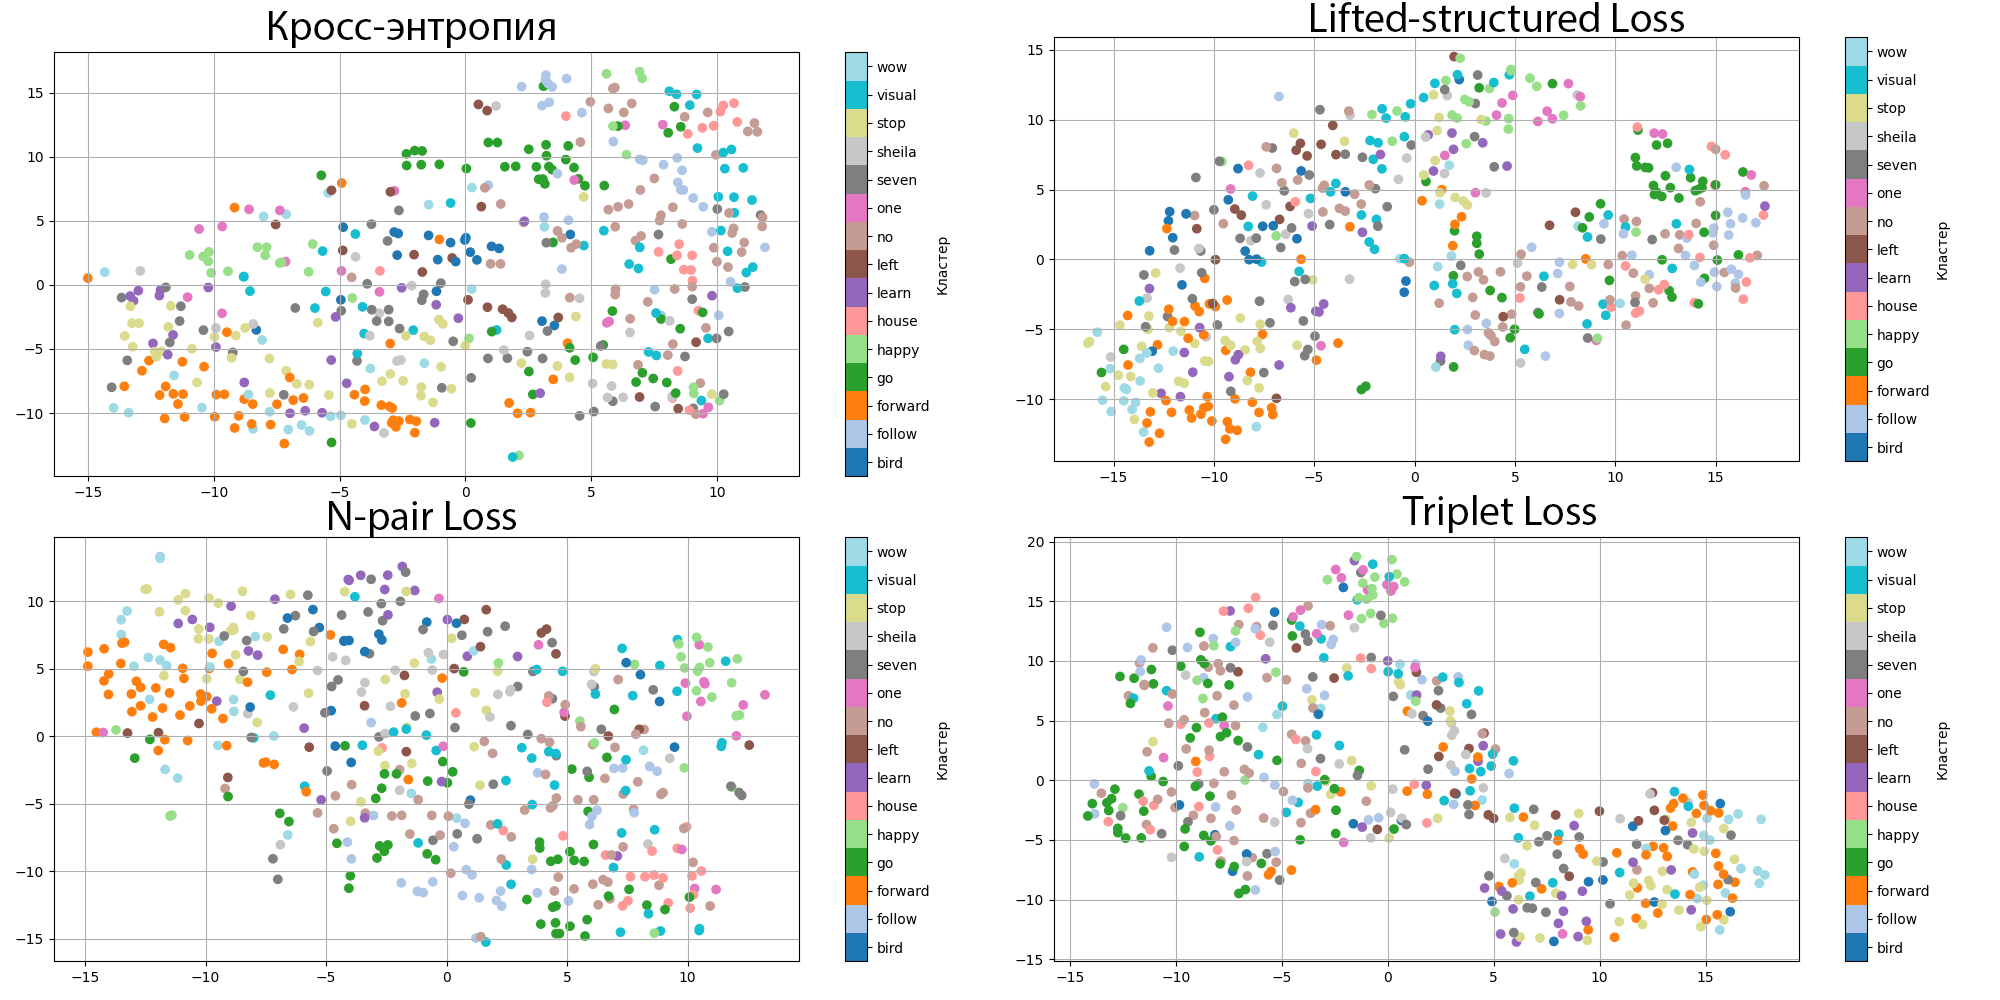
\includegraphics[width=16cm]{Images/test_tsne_4.png}
\label{fig:tsne_test_4}
\end{figure} % Эксперименты
\section{Выводы}
\label{sec:Chapter6} \index{Chapter6}

\par
В рамках работы было проведено исследование подходов к повышению эффективности обучения по нескольким примерам.
На основе обзора существующих методов к решению проблем FSL для исследования был выбран метод построения эмбеддингов с использованием различных функций потерь на примере задачи распознавания ключевых слов на датасете Google Speech V2, а также выбраны метрики оценки качества получаемого пространства эмбеддингов. Для проведения исследования были реализованы функции потерь Triplet Loss, Lifted Structured Loss, N-pair loss, а также базовая нейронная сеть, цикл обучения нейронных сетей и функции вычисления метрик кластеризации. Наиболее эффективной по выбранным критериям стала функция Lifted Structures Loss, которая показала на тестовом наборе по сравнению с другими результаты лучше: до 0.48 (31\%) по критерию FC и  до 0.04 (6\%) по критерию HV. %  Выводы 

\nocite{*}
\bibliographystyle{gost71u} % Для соответствия требованиям об оформлении списка литературы
\bibliography{references}

% \section*{Приложение}
\addcontentsline{toc}{section}{Приложение}
\label{sec:Apendix} \index{Apendix}

 

\end{document}
